\documentclass[10pt,a4paper]{article}
\usepackage[utf8]{inputenc}
\usepackage[T1]{fontenc}
\usepackage{amsmath}
\usepackage{amssymb}
\usepackage{graphicx}
\usepackage{float}
\title{Assignment \#3}
\author{Soulimane Mammar}
\begin{document}
	\maketitle
	\section*{Exercise 1}
	Write a program that prints a multiplication table, like this:
	
	\bigskip
	\begin{tabular}{cccccccccc}
		
		1 & 2 & 3 & 4 & 5 & 6 & 7 & 8 & 9 & 10 \\

		2 & 4 & 6 & 8 & 10 & 12 & 14 & 16 & 18 & 20 \\
		
		3 & 6 & 9 & 12 & 15 & 18 & 21 & 24 & 27 & 30 \\
		
		... &  &  &  &  &  &  &  &  &  \\
		
		10 & 20 & 30 & 40 & 50 & 60 & 70 & 80 & 90 & 100 \\
		
	\end{tabular}
	\section*{Exercise 2}
	Mean and standard deviation. Write a program that reads a set of floating-point data values. Choose an appropriate mechanism for prompting for the end of the data set. When all values have been read, print out the count of the values, the average, and	the standard deviation. The average of a data set $ \{x_1, \cdots, x_n\} $ is $ \bar{x} = \sum x_i / n $ , where	$ \sum x_i = x_1 +\cdots + x_n $ is the sum of the input values. The standard deviation is
	\begin{equation*}
		s = \sqrt{\dfrac{\sum (x-\bar{x})^2}{n}}
	\end{equation*}

	\section*{Exercise 3}
	Translate the following pseudocode for randomly permuting the characters in a string into a C++ program.
	\begin{itemize}
		\item Read a word.
		\item Repeat word.length() times
		\begin{itemize}
			\item Pick a random position i in the word.
			\item Pick a random position j > i in the word.
		\end{itemize}
		\item Swap the letters at positions j and i.
		\item Print the word.
	\end{itemize}
	To swap the letters, construct substrings as follows:
	\begin{figure}[H]
		\centering
		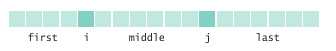
\includegraphics[width=0.7\linewidth]{assign3_fig1}
		\label{fig:assign3fig1}
	\end{figure}
	
	Then replace the string with
	
	\verb|first + word.substr(j, 1) + middle + word.substr(i, 1) + last|
	
	\section*{Exercise 4}
	The max function that is declared in the <algorithm> header returns the larger of its two
	arguments. Write a program that reads three floating-point numbers, uses the max 	function, and displays
	\begin{itemize}
		\item the larger of the first two inputs.
		\item the larger of the last two inputs.
		\item the largest of all three inputs.
	\end{itemize}
	
	\section*{Exercise 5}
	Write a function \verb|sort3(int& a, int& b, int& c)| that swaps its three arguments to
	arrange them in sorted order. For example,
	\begin{verbatim}
		int v = 3;
		int w = 4;
		int x = 1;
		sort3(v, w, x); // v is now 1, w is now 3, x is now 4	
	\end{verbatim}
	
	\section*{Exercise 6}
	Write a recursive function\\
	\verb|string reverse(string str)|\\
	that computes the reverse of a string. For example, \verb|reverse("flow")| should return
	"wolf".
	
	\section*{Exercise 7}
	Use recursion to implement a function \verb|bool find(string str, string match)| that tests whether \verb|match| is contained in \verb|str|:\\
	\verb|bool b = find("Mississippi", "sip"); // Sets b to true|
\end{document}